%%%%%%%%%%%%%%%%%%%%%%%%%%%%%%%%%%%%%%%%%%%%%%%%%%%%%%%%
%%%%%%%%%%%%%%%%%%%%%%%%%%%%%%%%%%%%%%%%%%%%%%%%%%%%%%%%
\section{Materials and Methods}
%%%%%%%%%%%%%%%%%%%%%%%%%%%%%%%%%%%%%%%%%%%%%%%%%%%%%%%%
%%%%%%%%%%%%%%%%%%%%%%%%%%%%%%%%%%%%%%%%%%%%%%%%%%%%%%%%
%
FIM 3 is a fully operational pipeline of software tools to help acquire datasets, cache hydrofabrics, produce FIMs, and evaluate results.
%
%%%%%%%%%%%%%%%%%%%%%%%%%%%%%%%%%%%%%%%%%%%%%%%%%%%%%%%%
\subsection{Software Dependencies and Architecture}
%%%%%%%%%%%%%%%%%%%%%%%%%%%%%%%%%%%%%%%%%%%%%%%%%%%%%%%%
%
OWP FIM exclusively utilizes free and open source software dependencies including Python 3, GDAL, TauDEM, Geographic Resource Analysis Support System (GRASS), GNU Parallel, and MPICH \cite{python382,gdal2020,tarboton2005terrain,grass2020,tange2015gnu,amer2021mpich}.
Within the Python 3 ecosystem, many common packages are employed including but not limited RichDEM, GeoPandas, Rasterio, Rasterstats, and Numba \cite{barnes2018richdem,jordahl2014geopandas,lam2015numba}. 
To simplify setup and enhance portability across host operating systems OWP FIM packages all dependencies up in Docker image (\url{https://docs.docker.com/engine/install/}). 
A user only need to install Docker on their host machine and build the image from the provided recipe. 

The FIM 3 pipeline is discretized into key areas that a user can interact with to reproduce the results of this study. Preprocessing acquires and prepares datasets for production of the FIM 3 hydrofabric. 
Producing the FIM hydrofabric produces the datasets required to make an inundation map including the relative elevation model (REM) or HAND grid, the catchments in vector and raster form, and the hydro-table (contains synthetic rating curves and cross-walk information).
%
%%%%%%%%%%%%%%%%%%%%%%%%%%%%%%%%%%%%%%%%%%%%%%%%%%%%%%%%
\subsection{Datasets}
%%%%%%%%%%%%%%%%%%%%%%%%%%%%%%%%%%%%%%%%%%%%%%%%%%%%%%%%
%
All data sources used within FIM 3 are publicly available from a variety of government sources including the USGS, NWC, Federal Emergency Management Agency (FEMA), and US Army Core of Engineers (USACE) to enhance reproducibility and collaboration among government, academia, and industry.
The National Hydrography Dataset Plus High Resolution (NHDPlusHR) Beta Version is the latest hydrography dataset used for land surface hydrologic modeling in the US \cite{moore2019user}. 
It is used in conjunction with the hydrofabric of the NWM V2.1 to help define flowlines for FIM 3 while the NWM hydrofabric is also used to define reservoirs for exclusion and catchments to cross-walk to for forecasting purposes.
The AHPS forecast points are required to determine the RnR downstream segments in order to define the RnR Mainstems (MS).
For enforcing levee data into the NED DEMs, the USACE National Levee Database (NLD) is used via burning feature elevations \cite{engineers2016national}.
Additionally, FEMA Base Level Engineering (BLE) from Region 6 (parts of Texas, Oklahoma, Arkansas, Louisiana and New Mexico) 1\% (100 year) and 0.2\% (500 year) datasets are used as validation in this study. 
These BLE datasets are provided at the watershed scale (HUC8) utilizing best available simulations and DEMs.
The full input datasets sorted by source are listed below:
%
\begin{enumerate}
\item{USGS - NHDPlusHR Beta}
    \begin{enumerate}
    \item{\textit{BurnLineEvents:} flowlines used by NHDPlusHR for hydro-enforcing DEM}
    \item{\textit{Value-Added Attributes:} database of additional attributes referenced to flowlines that enhance navigation, analysis, and display}
    \item{\textit{DEM:} DEM from National Elevation Dataset (NED) in 10m (or 1/3 arc-second) spatial resolution with vertical units in centimeters \cite{gesch2002national}}
    \end{enumerate}
\item{NOAA OWP - NWM V2.1 Hydrofabric}
    \begin{enumerate}
    \item{\textit{flowlines:} stream network center lines used for NWM routing and forecasting}
    \item{\textit{reach level catchments:} surface drainage area corresponding to each river reach}
    \item{\textit{waterbodies:} includes reservoirs, lakes, and others that are modeled within the NWM}
    \end{enumerate}
\item{USACE - NLD}
    \begin{enumerate}
    \item{\textit{Levee elevations:} Top of levee elevations are gathered with in the NLD provided by USACE for hydro-enforcement}
    \end{enumerate}
\item{Land Sea Border}
\item{FEMA BLE}
    \begin{enumerate}
    \item{\textit{cross-sections:} cross-sections and associated data for associating 1\% and 0.2\% recurrence discharges with NWM reaches}
    \item{\textit{flood inundation maps:} FIMs produced by BLE at the two recurrence intervals for comparison with FIMs from OWP FIM versions}
    \end{enumerate}
\item{NOAA OWP - AHPS Forecast Points}
    \begin{enumerate}
    \item{\textit{AHPS:} Collection AHPS forecast points to associate to RnR Mainstems}
    \end{enumerate}
\end{enumerate}
%
%%%%%%%%%%%%%%%%%%%%%%%%%%%%%%%%%%%%%%%%%%%%%%%%%%%%%%%%
\subsection{Hydro-conditioning}
%%%%%%%%%%%%%%%%%%%%%%%%%%%%%%%%%%%%%%%%%%%%%%%%%%%%%%%%
%
The DEM from the NED is subject to a series of hydro-conditioning procedures to enhance it's suitability for riverine flood inundation mapping. 
These techniques are specific for making OWP FIM and differ from the conditioning methods used by the NHDPlusHR Beta \cite{moore2019user}.
Hydro-conditioning is implemented to obtain many objectives including enforcing the location of hydrologically relevant features such as flowlines, lakes, or drainage divides whether natural or anthropogenic. 
It can also be used to simulate more accurate bathymetry which is not accounted for in the NED 10m DEM \cite{gesch2002national}.

Specifically within the context of FIM 3, the hydro-conditioning operations that take place in sequential order are presented. 
Prior to any hydro-conditioning, all input datasets must be subset from their original spatial domain scales into the processing unit designated at run time which can be either HUC 4, 6 or 8. 
The subsetting is done by spatial query for the cases of the levees, DEM, and NWM hydrofabric while the NHDPlusHR BurnLineEvents are subset via attribute query for the given reachcode's membership in the processing unit.
Hydro-conditioning raster operations take place on buffered boundary definitions to avoid edge contamination and effects \cite{lindsay2013measuring}. 
%
%%%%%%%%%%%%%%%%%%%%%%%%%%%%%%%%%%%%%%%%%%%%%%%%%%%%%%%%
\subsubsection{Stream Network Enforcement} 
\label{ssec:stream_network_enforcment}
%
\note[Fernando Aristizabal]{For Brian Avant}
The location of the stream network are enforced to ensure general agreement with established stream networks.
The NHDPlus HR Beta Burnline Event layer is used to enforce stream locations in the NHDPlusHR workflow so it is also used here for hydro-enforcement \cite{moore2019user}. 
However, to better match the drainage density of the NWM V2.1 stream network which is based on the NHDPlus Medium Resolution, the Burnline Events are pruned utilizing a nearest neighbor search around the NWM flowlines. 
Pruning the NHD network is completed at for every NWM V2.1 headwater point, the nearest NHDPlusHR Burline Event feature is selected and downstream features are also selected.
The resulting pruned NHD stream network is what gets hydro-enforced in subsequent operations.
This procedure is best illustrated in Figure \ref{fig:stream_density_pruning} which shows that the pruned NHD network corresponds to the full density NHD network at NWM V2.1 headwater locations only. 
Additionally, the NHDPlusHR pruned headwaters are later used for seeding a new FIM drainage network that best agrees withe DEM after all hydro-conditioning takes place.
%
\begin{figure}[h!]
\centering
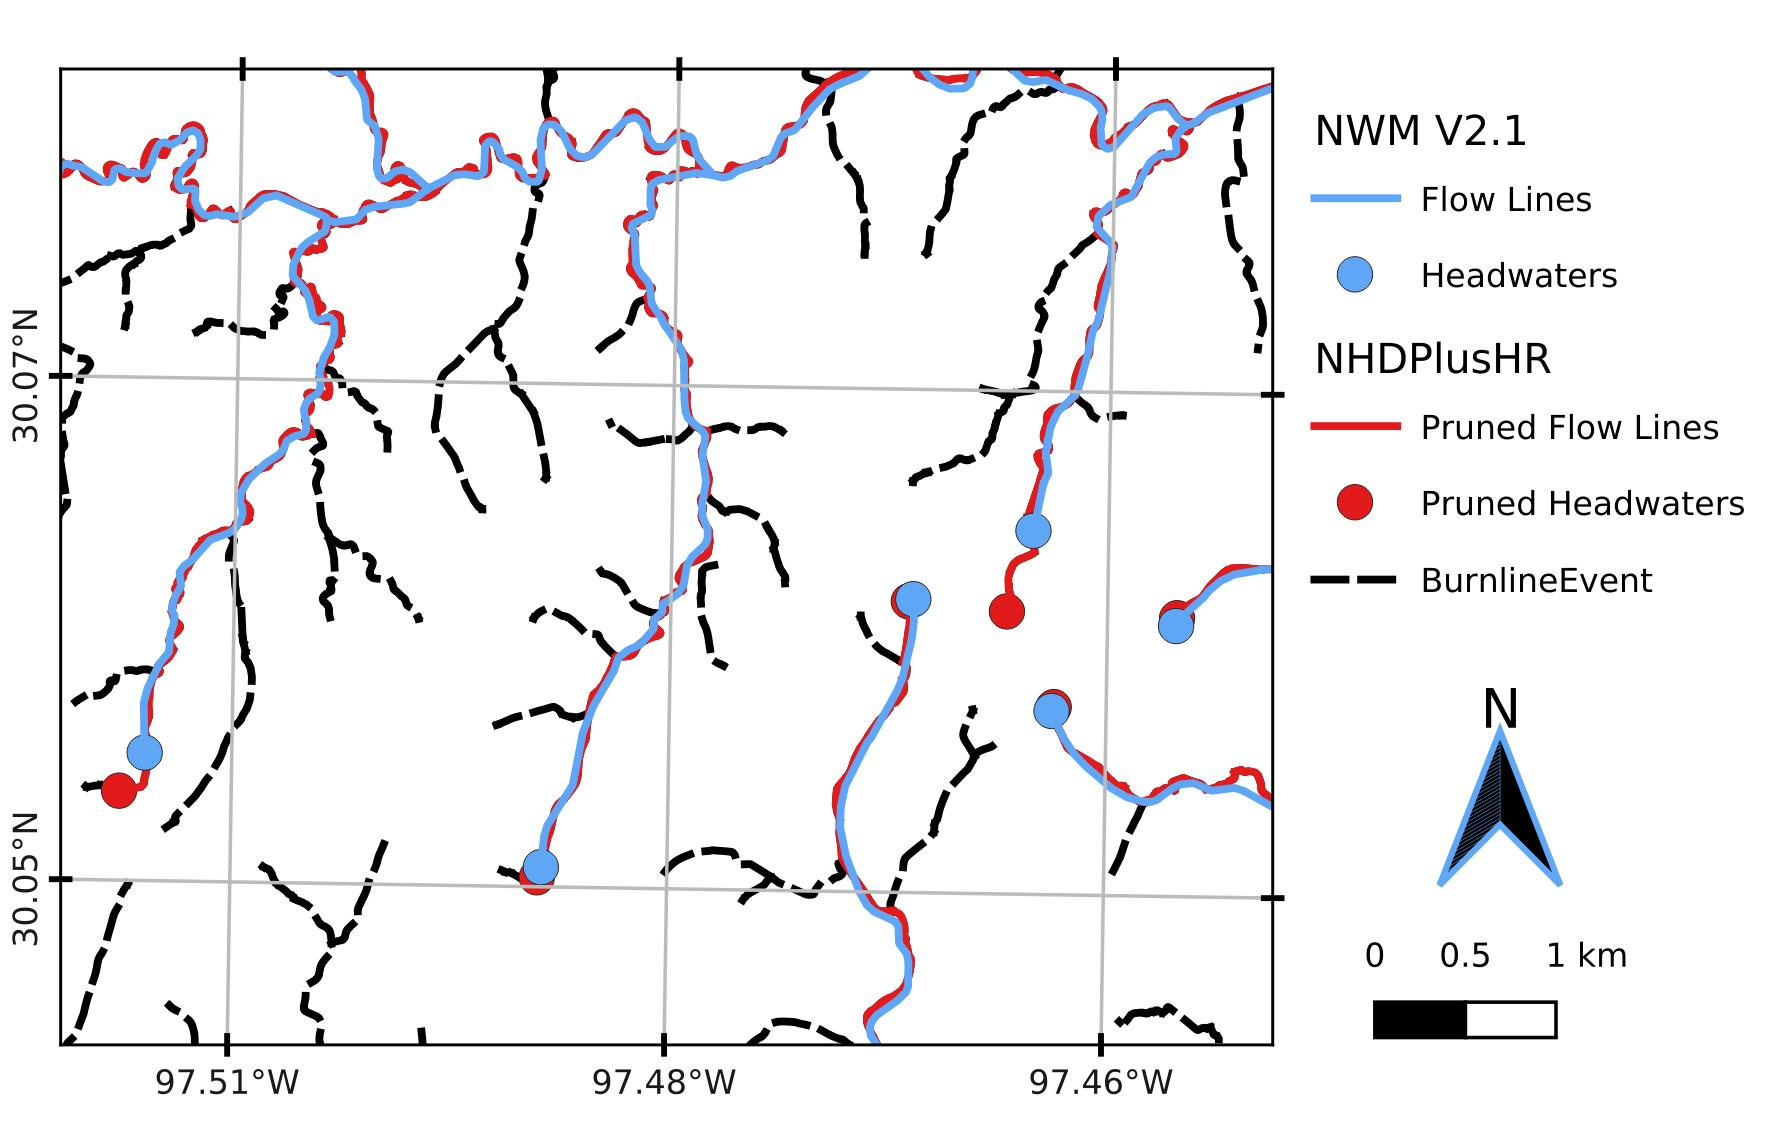
\includegraphics[scale=1.0]{figures/headwaters.jpg}
\caption{Pruning of NHDPlus HR Beta Burnline Events (dotted black) to NWM V2.1 stream density (blue) using nearest neighbor selection. Resulting stream network (red) matches the drainage density of NWM V2.1 while corresponding spatially with the NHDPlusHR Burnline Events.}
\label{fig:stream_density_pruning}
\end{figure}
%
This results in a stream network that has the same density as the NWM V2.1 flowline network but utilizes the locations of the NHDPlusHR Beta BurnLineEvents. 

\note[Fernando Aristizabal]{For Trevor Grout}
The pruned stream network is then utilized to hydro-enforce the DEM with a methodology developed by \citeA{hellweger1997agree} known as the AGREE DEM Surface Reconditioning System. 
The AGREE algorithm seeks to burn artificially deep thalweg elevations by a uniform value known as sharp drop. 
The modification continues by excavating an area of a given buffer distance from the thalweg by a depth proportional to the distance from the channel given by the smooth drop. 
The resulting enforcement of the thalweg and general bathymetric region results in a cross-section resembling a trapezoidal shape with a significantly lower elevation along the thalweg line only as can be seen in Figure \ref{fig:agree_dem_cross_section}.
%
\begin{figure}[h!]
\centering
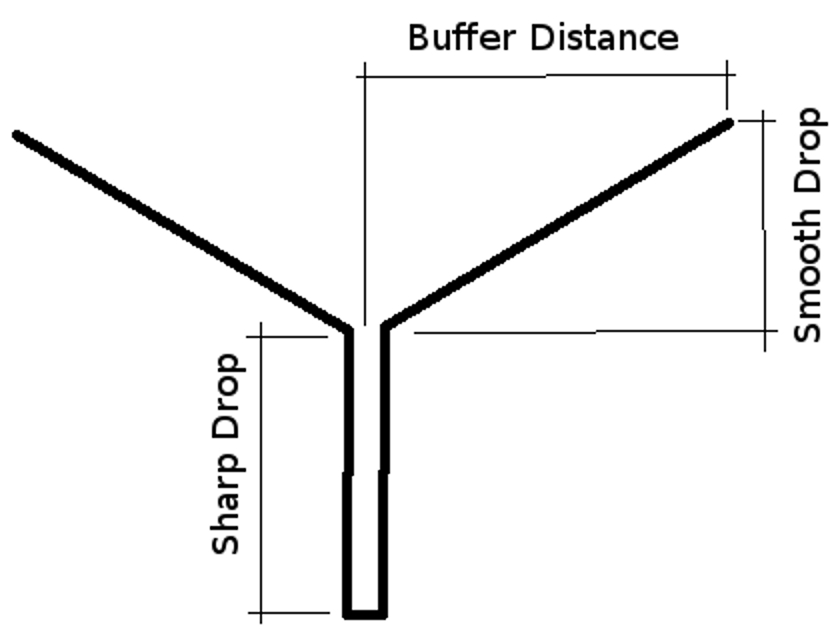
\includegraphics[scale=1.0]{figures/agree_dem_cross_section.jpg}
\caption{Placeholder for AGREE DEM illustration}
\label{fig:agree_dem_cross_section}
\end{figure}
%
In total, the AGREE algorithm requires three parameters including the buffer distance, smooth drop, and sharp drop. 
Using simple thalweg burning techniques as opposed to the full AGREE method helps prevent distortions in the delineation of streams as well as the catchment boundaries \cite{saunders1995grid,saunders1996gis,mizgalewicz1996modeling,hellweger1997agree,quenzer1998gis,baker2006comparison}.
\citeA{baker2006comparison} noted AGREE produced satisfactory results when compared to other enforcement especially when computational costs are considered. 
Downsides to the technique include the possibility of exhibiting parallel streams where the burned stream and real stream are both represented \cite{hellweger1997agree,saunders1999preparation} and some distortion of the catchment boundaries can also be observed \cite{saunders1999preparation,saunders1996gis}. Some of these drawbacks are later addressed by additional conditioning techniques later on.
%
%%%%%%%%%%%%%%%%%%%%%%%%%%%%%%%%%%%%%%%%%%%%%%%%%%%%%%%%
\subsubsection{Levee Enforcement}
%
\note[Fernando Aristizabal]{For Ryan Spies}
The National Elevation Dataset at 10m resolution lacks sufficient representation of fine grain features such as levees and embankments.
In order to better represent the influences of these features upon hydraulics and inundation extents, the National Levee Database (NLD) published by USACE was used to enforce elevations within the 10m DEM.
%
%\begin{figure}[h!]
%\centering
%\includegraphics[scale=1.0]{figures/levee_histogram.jpg}
%\caption{Placeholder for figure demonstrating histogram of elevation differences. May have too many results figures to allow for one}
%\label{fig:levee_histogram}
%\end{figure}
%
%%%%%%%%%%%%%%%%%%%%%%%%%%%%%%%%%%%%%%%%%%%%%%%%%%%%%%%%
\subsubsection{Depression Filling}
%
Local depressions are a naturally occurring features of a DEM but must be addressed if a connected drainage network with continuous catchments are to be derived for flood modeling purposes.
The conditioned DEM was removed of depressions by filling areas with pits while preserving the stream and levee information previously enforced.
Priority-Flood developed by \citeA{barnes2014priority} is an algorithm for filling said depressions and shown to have improved performance over early works in the field by \citeA{jenson1988extracting} implemented in \citeA{tarboton2005terrain} as well as \citeA{planchon2002fast}.
The depression filling algorithm used in our pipeline is a Priority-Flood variant developed by \cite{zhou2016efficient} with enhanced single-thread performance and a time complexity of O(n log n) for floating point grids.
This performance was enabled by limiting the processing queue with a region-growing method to exclude many of the slope cells \cite{zhou2016efficient}.
The depression technique employed here does leave the existence of flat regions where pits existed aprior thus later requiring the need for resolving these flats.
The enhanced variant of Priority-Flood is implemented and made available by \citeA{barnes2018richdem} and \citeA{zhou2015filldem}.
%
%%%%%%%%%%%%%%%%%%%%%%%%%%%%%%%%%%%%%%%%%%%%%%%%%%%%%%%%
\subsubsection{Stream Thalweg Elevation Conditioning}
%
Thalweg elevations are critical components of relative elevation based inundation mapping thus much is performed to ensure the best available, monotonically decreasing elevations are derived prior to normalizing of elevations.
In order to prevent situations where the burned thalweg and the thalweg endemic to DEM run parallel to one another, the normalized excavation algorithm \cite{saunders1999preparation} is used to seek a zonal (nearest neighbor) elevation minimum for each thalweg pixel. 
Each zone is defined as the thalweg's pixel nearest neighborhood within a maximum distance of 50m.
The zonal minimum is computed for each thalweg pixel zone and the minimum is used to replace the existing thalweg elevation value.

The next step involves conditioning these local minimums along the thalweg to enforce monotonically decreasing thalweg elevations for FIM.
\citeA{garousi2019terrain} proposed an algorithm that traverses stream thalweg pixels in a depth first manner starting with adding all the headwater pixels to a queue. 
The connectivity of the thalweg pixels is defined by the D-8 flow directions further discussed in Section \ref{ssec:flow_direction_and_flat_resolution}.
At every thalweg pixel, the minimum elevation among itself and its upstream contributing thalweg pixels is taken as shown in equation \ref{eq:thalweg_breach},
%
\begin{equation}
\label{eq:thalweg_breach}
\textbf{D}[x] = \min_{y\ drains\ to\ x} {(\ \textbf{D}[x]\ ,\ \textbf{D}[y]\ )}
\end{equation}
%
, in which \textbf{D} represents the array of thalweg adjusted elevations indexed by x and y where by y is upstream of x. 
When a pixel's upstream neighbors are all evaluated, the downstream pixel is added into the queue thus the depth first traversal of the drainage network.
This procedure enforces the location of streams and ensures that thalweg elevations are hydrologically correct which yielded a 7\% improvement in critical success index (CSI) per an evaluation for an event in 2017 on the Malad river \cite{garousi2019terrain}.
%
%%%%%%%%%%%%%%%%%%%%%%%%%%%%%%%%%%%%%%%%%%%%%%%%%%%%%%%%
\subsection{Deriving FIM Hydrofabric}
%%%%%%%%%%%%%%%%%%%%%%%%%%%%%%%%%%%%%%%%%%%%%%%%%%%%%%%%
%
%%%%%%%%%%%%%%%%%%%%%%%%%%%%%%%%%%%%%%%%%%%%%%%%%%%%%%%%
\subsubsection{Flow Directions and Flats Resolution}
\label{ssec:flow_direction_and_flat_resolution}
%
To facilitate the generation of a connected stream network and its associated catchments from the conditioned DEM, the depression-filled DEM is used to derive connectivity in the form of D-8 flow directions.
D-8 seeks to allocate a drainage direction for every pixel based on the adjacent eight pixel neighborhood with the steepest slope \cite{o1984extraction}.
The horizontal component of slope is defined as one for the 4 neighboring pixels in the main cardinal directions while the intercardinal pixels are designated a horizontal component of square root of 2. 
The flow direction is encoded as integers 1 through 8 corresponding with the cardinal direction East as 1 and continuing counter-clockwise to the Southwest direction as 8. 
Flow directions are derived for non-depression filled regions trivially with the above procedure but to define connectivity for every grid cell the remaining flats corresponding to depression filled cells must be resolved.

Flat resolution from flats endemic to the DEM or from depression filled regions is a costly,non-trivial procedure which was originally addressed by \citeA{garbrecht1997assignment}.  
Software implementations have developed means to partition the problem and resolve flats iteratively with communication across processes \cite{tarboton2009generalized,tesfa2011extraction,wallis2009parallel,tarboton2005terrain}.
The excessive iteration and communication leads to poor computational performance which motivated further work on how to optimize flat resolution \cite{survila2016scalable,barnes2014efficient}.
Specifically the work by \citeA{survila2016scalable} enables the use of parallel processing and made smoother catchments from our informal experience than those from \citeA{barnes2014efficient}.
By processing flats local to each partition separately from flats shared with other partitions, the accelerated flat resolution algorithm demonstrated an average speed up 468x when compared to prior implementations \cite{survila2016scalable}.
OWP FIM 3 utilized a CyberGIS implementation of the D-8 flow direction algorithm with the accelerated resolution of flats \cite{survila2016scalable,cybergis2016}.
%
%%%%%%%%%%%%%%%%%%%%%%%%%%%%%%%%%%%%%%%%%%%%%%%%%%%%%%%%
\subsubsection{Deriving FIM Stream Network}
%
\note[Fernando Aristizabal]{For Brian Avant}
The derivations of relative elevations and catchments from the newly conditioned DEM involves re-deriving a new FIM stream network. 
The FIM stream network is of the same density as the NWM V2.1 network and fully converges at all junctions leaving no divergences in the network.
This is accomplished by using the seed points generated from the stream network enforcement process (Section \ref{sec:stream_network_enforcment}).
These seeds points are headwater locations of the NHDPlusHR Beta Burnline Events layer that spatially correspond to theheadwater definitions in the stream network of the NWM V2.1.

Additionally, each stream link in the FIM stream network is split into equidistant reaches
Stream links are defined here as segments of rivers discretized by junctions with other NWM river segments or NWM lakes.
D-8 flow accumulation from seed points, thresholding, conversion to vector, splitting to equal lengths at junctions and lakes, globally unique reach id's based on HUC 8 id, cross-walking
\cite{wallis2009parallel}
%
%%%%%%%%%%%%%%%%%%%%%%%%%%%%%%%%%%%%%%%%%%%%%%%%%%%%%%%%
\subsubsection{Catchments}
%

%
%%%%%%%%%%%%%%%%%%%%%%%%%%%%%%%%%%%%%%%%%%%%%%%%%%%%%%%%
\subsubsection{Relative Elevation Model}
%

%
%%%%%%%%%%%%%%%%%%%%%%%%%%%%%%%%%%%%%%%%%%%%%%%%%%%%%%%%
\subsubsection{Synthetic Rating Curves}
%

%
%%%%%%%%%%%%%%%%%%%%%%%%%%%%%%%%%%%%%%%%%%%%%%%%%%%%%%%%
\subsection{RnR Mainstems Method}
%

%
%%%%%%%%%%%%%%%%%%%%%%%%%%%%%%%%%%%%%%%%%%%%%%%%%%%%%%%%
\subsection{Inundation Mapping}
%

%
%%%%%%%%%%%%%%%%%%%%%%%%%%%%%%%%%%%%%%%%%%%%%%%%%%%%%%%%
\subsection{Evaluation and Testing}
%%%%%%%%%%%%%%%%%%%%%%%%%%%%%%%%%%%%%%%%%%%%%%%%%%%%%%%%
%

%
